\documentclass[12pt,serif,hyperref={CJKbookmarks=true}]{beamer}
\usepackage[space,noindent]{ctex}
\usepackage[lined,commentsnumbered]{algorithm2e}
%beamer settings
\useoutertheme{infolines}
\useinnertheme{rounded}
\usefonttheme{default}
\usecolortheme{rose}

\renewcommand{\tablename}{表}
\begin{document}
  \kaishu
  \title[2013.5.17]{可视化的Java多线程程序错误定位工具}
  \subtitle{Visual Fault Localization Tool for Java Multi-threaded Program}
  \author{黄亚铭\quad 指导老师:孙玉霞}
  \institute{暨南大学计算机系}
  \date[毕业论文答辩]{暨南大学本科生毕业设计(论文)答辩}
  \logo{
\includegraphics[width=.1\textwidth]{jnu.jpg}}

  \setbeamercolor{up}{fg=white,bg=purple}
  \setbeamercolor{low}{fg=black,bg=pink}

  \begin{frame}
    \titlepage
  \end{frame}

  %\begin{frame}
  %  \frametitle{要点}
  %\end{frame}

  \section{课题背景}
  \subsection{程序的并发错误}
  \begin{frame}
    \frametitle{并行程序的难点}
    \begin{enumerate}
      \item 编写并行程序比编写串行程序更加困难(死锁、数据争用\ldots)
      \pause
      \item 测试并行程序比测试串行程序更加困难
      \begin{itemize}
        \item 难以重现错误
        \item 不易定位
      \end{itemize}
    \end{enumerate}
  \end{frame}

  \subsection{Falcon}
  \begin{frame}
    \frametitle{Falcon}
    \begin{itemize}
      \item Fault Localization in Concurrent Programs
      \item Sangmin Park, \textit{et al.}
    \end{itemize}
  \end{frame}

  \begin{frame}
    \frametitle{错误类型的划分}
    \begin{block}{数据访问模式(Data Access Pattern)}
      如果在并发程序运行的过程中,不同线程访问共享数据的方式符合这些数据访问模式,就有出现并发错误的可能性。
    \end{block}
    \pause
    \begin{exampleblock}{顺序破坏(Order Violation)}
      访问一个共享变量的两个线程(其中一个线程进行写操作)因为访问顺序交错导致读、写错误的数据。
    \end{exampleblock}
    \begin{exampleblock}{原子性破坏(Atomicity Violation)}
      一个线程操作共享变量的过程中,另外一个线程操作被错误的插入。
    \end{exampleblock}
  \end{frame}

  \begin{frame}
    \frametitle{Falcon工作流程}
    \centering
    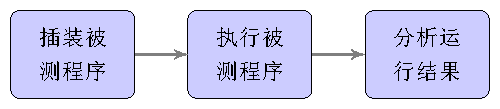
\includegraphics[width=\textwidth]{FlowDiagram.pdf}
  \end{frame}

  \begin{frame}
    \frametitle{插装被测程序}
    插装的难点:
    \begin{enumerate}
      \item 如何判断变量是否被多个线程访问?
      \item 如何判断变量是读还是写?
      \item 如何插入探针?
    \end{enumerate}
    \pause
    解决方法:Soot
    \begin{enumerate}
      \item 使用Soot进行线程逃逸分析
      \item 使用Jimple分析语句中的变量
      \item 使用Soot API插入探针,并生成.class文件
    \end{enumerate}
  \end{frame}

  \begin{frame}
    \frametitle{运行被测程序}
    \textbf{多次}运行经过插装的被测程序。
    \pause
    \begin{itemize}
      \item 识别数据访问模式
      \item 记录数据访问模式和运行结果(序列化为XML文件保存)
    \end{itemize}
  \end{frame}

  \begin{frame}
    \frametitle{统计运行结果}
    \framesubtitle{Jaccard系数}
    对于一个数据访问模式$p$,有通过的执行数$pass(p)$,失败的执行数$failed(p)$和该被测程序所有测试失败的个数$totalfalied$,可以得到可疑度:
    \begin{equation*}
      suspiciousness(p)=\frac{failed(p)}{totalfailed + passed(p)}
    \end{equation*}
  \end{frame}

  \section{Falcon的实现}
  \subsection{我的工作}
  \begin{frame}
    \frametitle{我的工作}
    \begin{beamerboxesrounded}[upper=up,lower=low,shadow=true]{对Falcon的补充和改进}
      \begin{enumerate}
         \item 补充代码
         \pause
         \item 完善算法
         \pause
         \item 重构
         \pause
         \item 可视化
      \end{enumerate}
    \end{beamerboxesrounded}
  \end{frame}

  \subsection{Falcon的可视化}
  \begin{frame}
    \frametitle{效果截图}
    \framesubtitle{顺序破坏}
    \centering
    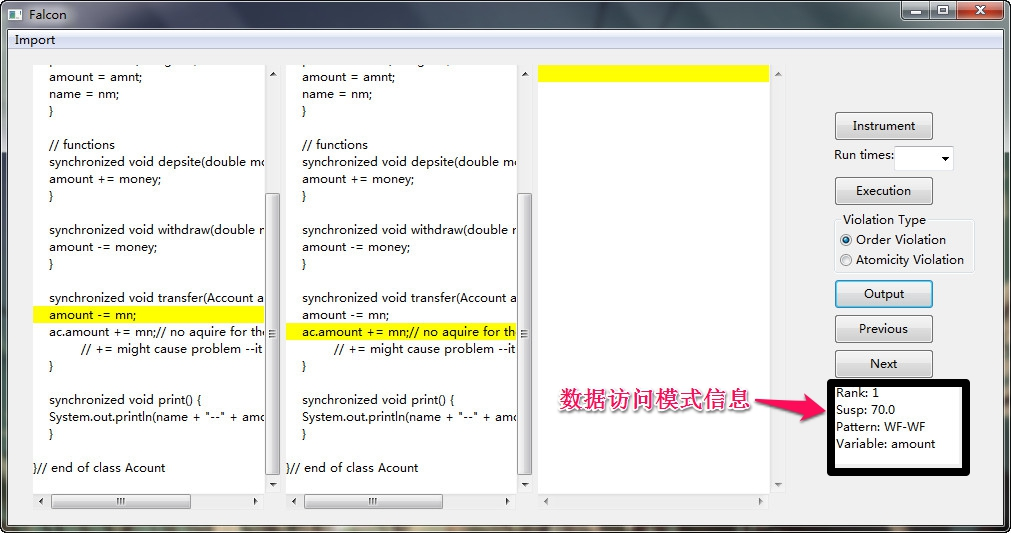
\includegraphics[width=.8\textwidth]{order.jpg}
  \end{frame}

  \begin{frame}
    \frametitle{效果截图}
    \framesubtitle{原子性破坏}
    \centering
    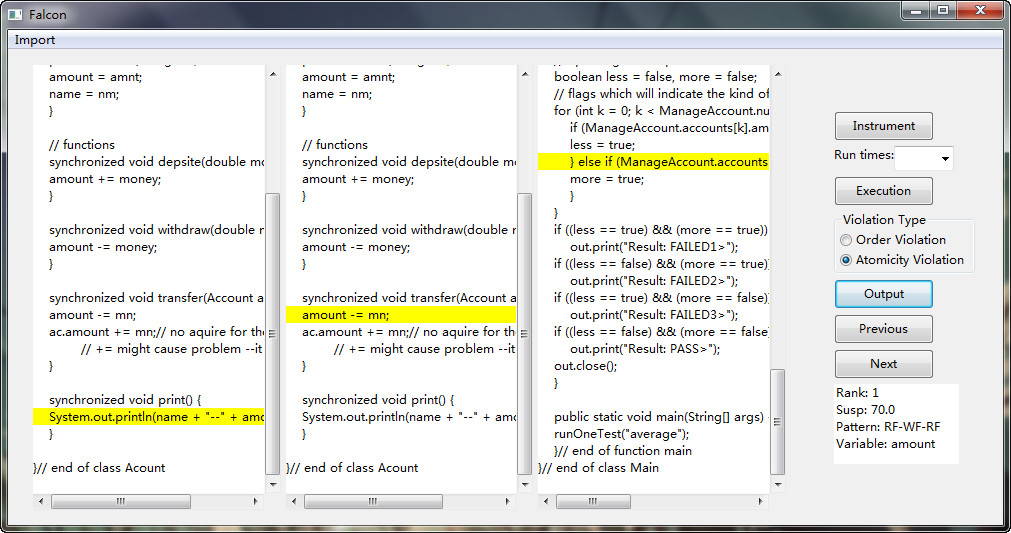
\includegraphics[width=.8\textwidth]{atom.jpg}
  \end{frame}

\end{document}
